\documentclass[12pt,a4paper]{article}
\usepackage[latin1]{inputenc}
\usepackage[spanish]{babel}
\usepackage{graphicx}
\usepackage[left=1.3cm,right=1.3cm,top=1.8cm,bottom=4cm]{geometry}
\usepackage{lastpage}
\usepackage{marginnote}
\usepackage{multirow}
\usepackage{wallpaper}
\usepackage{fancyhdr}
\setlength{\headheight}{87pt} 
\pagestyle{fancy}\fancyhf{}
\renewcommand{\headrulewidth}{0pt} 
\setlength{\parindent}{0cm}
\newcommand{\tab}{\hspace*{2em}}
\newcommand\BackgroundStructure{
	\setlength{\unitlength}{1mm}
	\setlength\fboxsep{0mm}
	\setlength\fboxrule{0.5mm}
	\put(10, 10){\fcolorbox{black}{white!10}{\framebox(192,247){}}}
	\put(10, 262){\fcolorbox{black}{white!10}{\framebox(192, 31){}}}
}

%-------------------------ENCABEZADO---------------
\fancyhead[L]{\begin{tabular}{l r | l r}	
		\textbf{Proyecto} & 1 & \textbf{Página} & \thepage/\pageref{LastPage} \\
		\textbf{Trabajo} & Desarrollo de un controlador & \textbf{Actualizado en:} & 27/08/2016 \\
		\textbf{} &  VGA & \textbf{Revisado en:} & 30/08/2016 \\
		\textbf{Grupo} & 1 & \textbf{Diseñadores} & Keylor Mena Venegas \\
		\textbf{Revisado por:} & Alfonso Chacón Rodríguez & \textbf{ } & Luis Leon Vega \\
		\textbf{} & & \textbf{ } & Luis Merayo Gatica
	\end{tabular}}
	
	\begin{document}
		\AddToShipoutPicture{\BackgroundStructure}
		
		\section*{\textit{Resumen}}
		
		Se debe realizar un controlador para realizar la lectura y escritura del módulo RTC V3023. Los datos del sistema deben poder ser desplegados en un monitor LCD mediante el protocolo VGA. Ante ello, se debe realizar un controlador para el RTC y para la VGA. Asimismo, se deben poder ajustar la hora, activar la alarma y el cronómetro de forma descendente mediante botones e interruptores dispuestos en la FPGA Nexys 4.\\
		
		\section*{\textit{Introduccion}} 
		Este proyecto consiste en realizar un controlador de módulos RTC (Real Time Controller), específicamente para el módulo V3023. Este controlador será capaz de escribir y leer dicho módulo para obtener parámetros de reloj, cronómetro y alarma. \\
		Asimismo, para poder desplegar la información relevante de los parámetros anteriores, se conectará un monitor LCD mediante el protocolo VGA. Por otro lado, para poder programar y dar instrucciones al circuito, se deberán usar los botones señalados en el instructivo y algunos interruptores. \\
		Finalmente, el conjunto es un circuito que permita controlar el módulo y comunicar al usuario mediante los botones y el monitor LCD, donde él podrá recibir la información relevante y poder modificar dicha información.\\
		
		\section{Objetivos}
		\begin{itemize}
			\item Diseñar un controlador de RTC que permita leerlo y programarlo mediante una interfaz de usuario consistente en botones incorporados dentro de la FPGA (Nexys 4) y un monitor comunicado a través del protocolo VGA.
			\item Investigar el funcionamiento del módulo RTC y el protocolo de comunicación del mismo.
			\item Diseñar un controlador para el módulo RTC, cuyo bus de datos y direcciones estén multiplexados.
			\item Cumplir con las reglas de temporizado del sistema, en especial, con el protocolo de comunicación del módulo RTC.
			\item Combinar el controlador de RTC con un controlador VGA para poder desplegar la información del módulo al usuario. Este módulo VGA será adaptado del proyecto anterior.
			\item Desarrollar un banco de pruebas (testbench) para poder emular el comportamiento del módulo RTC con la finalidad de comprobar el funcionamiento del circuito controlador.
		\end{itemize}
		
		\section{Descripción del sistema}
		El sistema se puede dividir en cuatro subsistemas, para facilitar el diseño dividimos el sistema en 4 grandes partes, el controlador de la pantalla, el controlador para el RTC, el control de usuario y  una memoria principal. Éstos subsistemas, pueden ser desarrollados de manera separada siempre que se tenga el cuidado necesario con los datos que comparten entre los bloques, para este efecto se desarrollo una memoria con 2 registros que se actualizan entre ellos al activar banderas. En la Fig. \ref{fig:sistema} se puede observar la composición general del sistema. \\[2ex]
		
		\begin{figure}[hbtp]
			\centering
			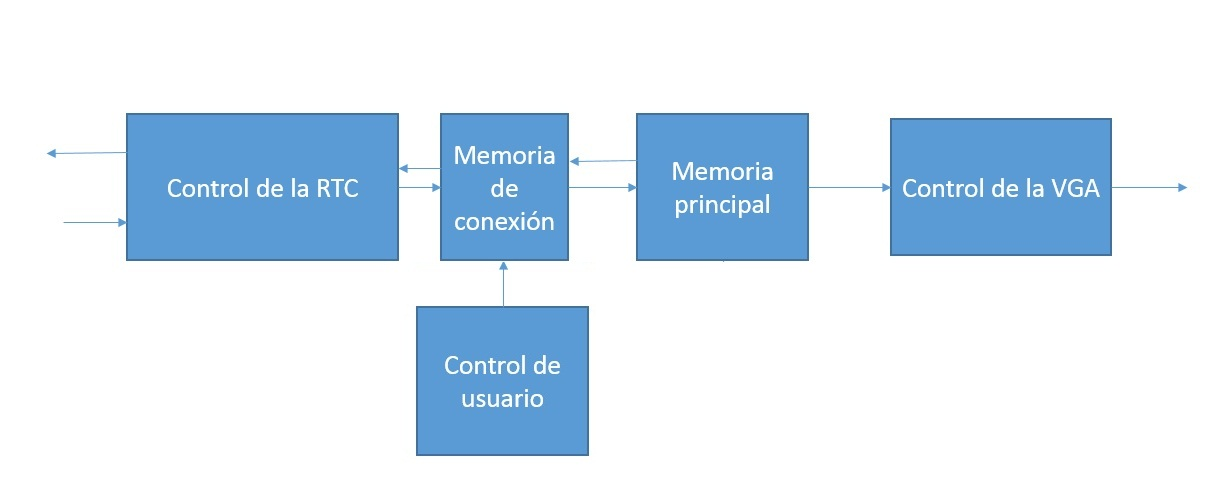
\includegraphics[height=8.5cm, width=18cm]{img/Subsistemas.jpg}
			\caption{Diagrama de modulos principales del sistema.}
			\label{fig:sistema}
		\end{figure}
		
		\subsection{Controlador de la pantalla}
		Para el periférico de despliegue de datos se ha solicitado emplear un monitor LCD controlado mediante el protocolo VGA (Video Graphics Array), con la finalidad de aprovechar el desarrollo del proyecto anterior y adaptando algunas cosas para poder incorporar datos dentro de la imagen que se desplegará en el monitor.
		\subsubsection{Diagrama de primer nivel}  \label{sec:VGA_pn}
		Para efectos del circuito, este debe tener acceso a los datos procedentes del buffer de memoria que contendrá la información que emite el RTC. Para ello, se ha puesto un banco de 16 registros (11 aprovechados) direccionados mediante un bus de direcciones de 4 bits y 8 bits de datos. Asimismo, se deben colocar las entradas y salidas pertinentes del protocolo, que son las salidas de sincronía y las salidas de color. \\[2ex]
		
		\begin{figure}[hbtp]
			\centering
			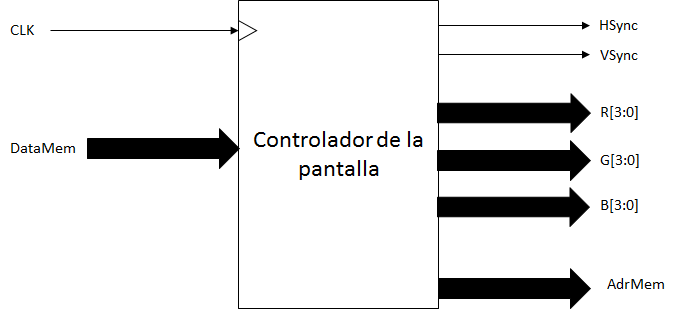
\includegraphics[width=15cm]{img/VGAPrimerNivel.png}
			\caption{Diagrama de primer nivel VGA}
			\label{fig:vgaPrimerNivel}
		\end{figure}
		
		A como es posible observar en la figura \ref{fig:vgaPrimerNivel}, existen dos buses que permiten obtener la información que será desplegada en la pantalla. El bus "AdrMem" permite direccionar el registro de la memoria de datos al registro que va a ser refrescado y el bus "DataMem" recopila la información del registro direccionado mediante "AdrMem". Esta comunicación es de solo lectura y solo será efectuada durante la sincronía vertical, que no contiene imagen para evitar glitches y cambios en el registro inesperados que vayan a afectar la nitidez de la imagen. \\[2ex]
		Para concluir este apartado, la interfaz se definirá mediante imágenes para cargar una interfaz agradable al usuario, esto aprovechando la capacidad de síntesis de memoria ROM en el entorno de Xilinx. \\[2ex]
		
		\subsubsection{Diagrama de segundo nivel} \label{sec:VGA_sn}
		Adentrando en el diseño, se pueden identificar tres grandes bloques que componen el control de pantalla, donde es posible generar los datos, generar las señales de posición y sincronía y las señales de los colores.
		
		\begin{figure}[hbtp]
			\centering
			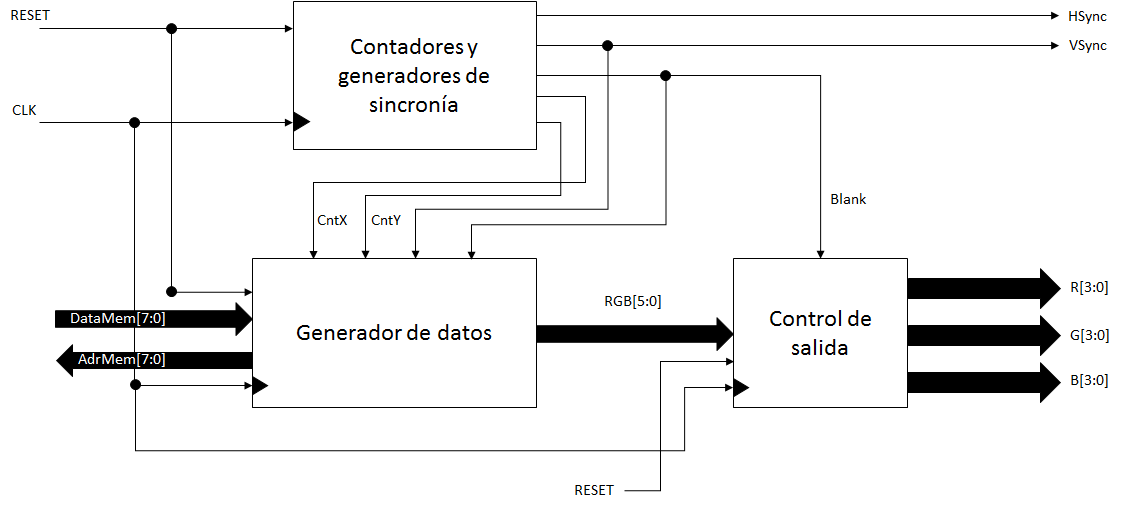
\includegraphics[width=18cm]{img/VGASegundoNivel.png}
			\caption{Diagrama de primer nivel VGA}
			\label{fig:vgaSegundoNivel}
		\end{figure}
		
		Como es posible apreciar en la figura \ref{fig:vgaSegundoNivel}, el primer bloque es el de "Contadores y generadores sincronía", que permite generar las señales de sincronización del monitor LCD y, además, generar la posición de la pantalla en la que se ubica el cursor. Esto último es clave para la etapa de "Generador de datos", que decidirá los datos que serán pintados y las memorias que serán consultadas. \\[2ex]
		
		El bloque "Generador de datos" permitirá producir las señales de color primitivo (2 bits por color) de la imagen que será pintada en la pantalla con base a los datos que se registren mediante los buses "AdrMem" y "DataMem", cuyos datos se almacenarán en un buffer de memoria de video. Basado en los datos de este buffer, se determinará el dato que se ilustrará (número) mediante un posicionamiento en memoria. Los datos que saldrán en la dirección serán generados por un contador de 12 dígitos y su proceso de incremento estará condicionado por el VSync para poder actualizar el buffer en momentos de sincronía, donde se no pintan pixeles. Por otro lado, las posiciones de memoria serán determinantes para consultar la memoria ROM que contendrá la interfaz y los números. \\[2ex]
		Por otro lado, el "Control de salida" permite decodificar el color en 2 bits en 4 bits mediante el duplicado. Asimismo, apaga los bits de salida en caso de entrar en etapa de sincronía, indicado mediante la entrada de "Blank". Esto evitará enviar datos en caso de ubicarse en un proceso de tiempo prohibido en la pantalla. \\[2ex]
		
		
		\subsubsection{Diagrama de tercer nivel}
		Profundizando aún más en el diseño, los bloques se pueden descomponer más haciendo evidente la presencia de una memoria ROM que contiene la información de la interfaz gráfica de usuario, que está subdividida en la memoria ROM de interfaz y la memoria ROM de los números, ya que todo el entorno es visual (véase figura \ref{fig:vgaTercerNivel}).\\[2ex]
		Asimismo, el generador de datos está compuesto por un direccionador de memoria mediante punteros y un banco de registros que ayudan a tener los datos estables para su uso. Dependiendo de la posición del cursor en la pantalla (CntX) y (CntY) y los datos de los registros, es posible direccionar a un campo específico de la memoria ROM de números y hacer el intercambio entre ROM de interfaz y ROM de números.\\[2ex]
		
			\begin{figure}[hbtp]
				\centering
				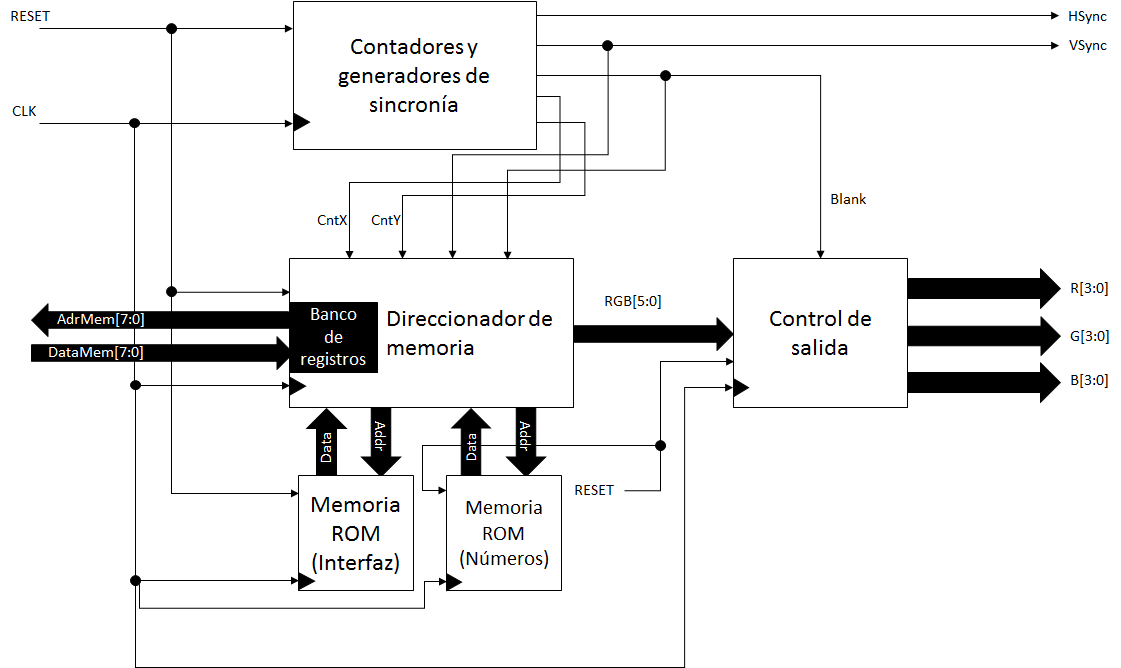
\includegraphics[width=18cm]{img/VGATercerNivel.png}
				\caption{Diagrama de primer nivel VGA}
				\label{fig:vgaTercerNivel}
			\end{figure}
			\begin{figure}[hbtp]
				\centering
				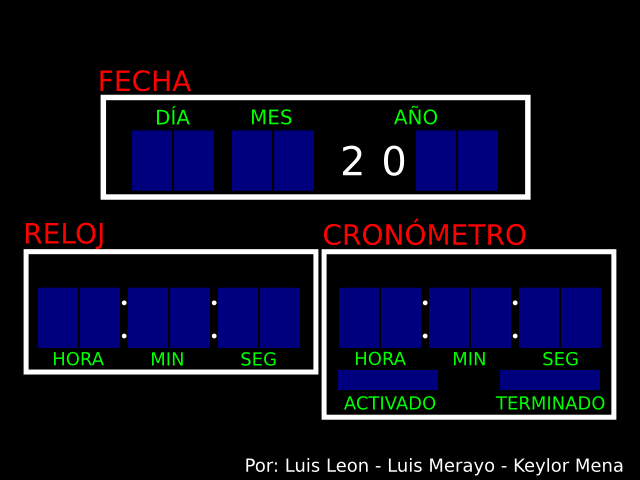
\includegraphics[width=13cm]{img/VGAInterfaz.png}
				\caption{Diagrama de primer nivel VGA}
				\label{fig:vgaInterfaz}
			\end{figure}
		
		Por otro lado, se encuentran los contadores y generadores de sincronía, que están compuestos por dos contadores y un bloque combinacional. El primer contador gobierna el conteo horizontal (CntX) y, a su vez, regula la velocidad de conteo descartando los 2 primeros bits menos significativos, por lo cual, el contador es de 12 bits para abarcar las 800 líneas horizontales. Este contador envía una señal de conteo al contador vertical, quien gobierna la posición vertical (CntY). El bloque combinacional permite generar las señales VSync y HSync dependiendo de la magnitud del conteo CntX y CntY, así como, la señal de Blank, donde no debe existir señal de color por encima de 0V.\\[2ex]
		El Control de salida permite, a como se explicó en el apartado anterior, expandir los bits de color para poder generar una señal de 12 bits de color. Asimismo, es gobernado por el Blank que pone en ceros todos los bits de color en tiempos de zona prohibida. \\[2ex]
		Para finalizar, las memorias tienen un dimensionamiento de 307200 espacios de memoria para albergar la interfaz de usuario (640X480) (figura \ref{fig:vgaInterfaz}) y de 24000 espacios para albergar las imágenes de los números (figura \ref{fig:vgaNumeros}). Los datos de estas memorias serán generadas por un script de Matlab y se cargarán mediante un archivo de texto con 6 bits. \\[2ex]
		
		
		\begin{figure}[hbtp]
			\centering
			
\includegraphics[width=1cm]{img/VGANumeros.png}
			\caption{Diagrama de primer nivel VGA}
			\label{fig:vgaNumeros}
		\end{figure}
		
		Cabe destacar que, la interfaz tiene espacios azules para indicarle al sistema de punteros cuando debe hacer cambio de imagen por un número. Esto se hizo con la finalidad de ahorrar espacio en la Nexys y optimizar el código, ya que existieron problemas debido al rendimiento en tiempo de todo el bloque VGA.\\[2ex]
		
		\subsection{Control de usuario}
		Para poder controlar el acceso del usuario, que se comunica por medio de 3 botones que indican que se quiere cambiar, el reloj, el timer o la alarma, y para moverse entre los registros de datos y aumentar o disminuir sus valores y 3 interruptores que [ermiten realizar estos cambios.\\ 
		
		\subsubsection{Diagrama de primer nivel}
		el control de usuario posee 3 interruptores y 3 botones para que el usuario elija los datos y que desea cambiar. Ademas posee entradas y salidas de memoria para poder alterar los registros y escribirlos en la rtc. Se puede notar esto en la figura \ref{fig:PrimerNivelcontrolusr}.
		
		\begin{figure}[htbp]
			\centering
			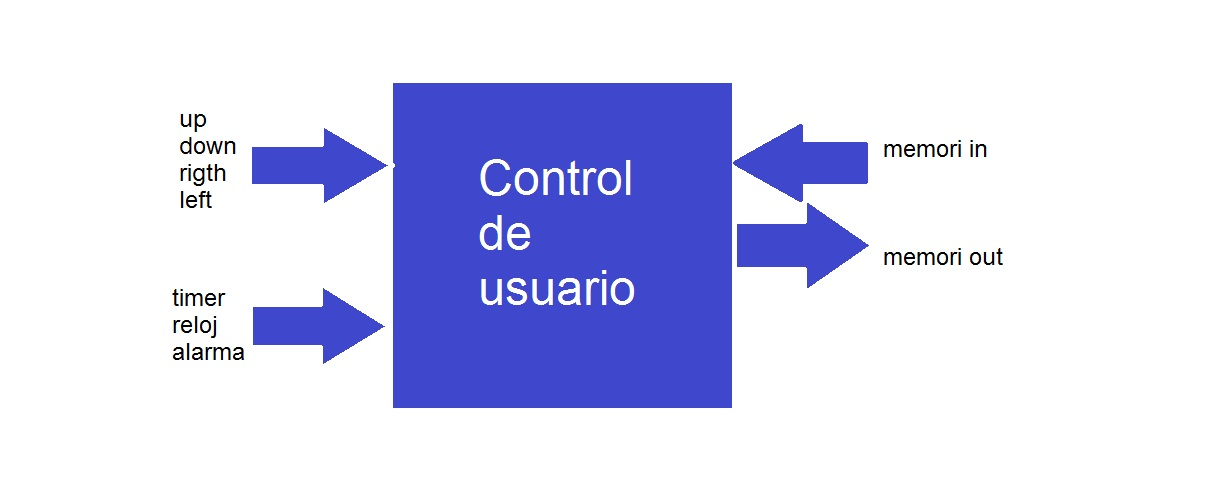
\includegraphics[height=3cm, width=10cm]{img/nivel1_contusr.jpg}
			\caption[1erNivel]{Diagrama de primer nivel del control de usuario.}
			\label{fig:PrimerNivelcontrolusr}
		\end{figure}
		
		\subsubsection{Diagrama de segundo nivel}
		En este diagrama mostrado en la Fig. \ref{fig:SegundoNivelControlusr} se muestra como se pretende realizar el control de usuario, el cual consiste en tan solo dos bloques.\\[2ex]
		
		Consiste un un control de acceso que controla el cambio de los valores de los registros y el control de sus direcciones en el registro. El registro almacenara los cambios que se desean realizar en la memoria y una etapa de salida que controla los momentos donde se escribe en la rtc los cambios que se desean en la rtc.\\[2ex]
		
		
		\begin{figure}[htbp]
			\centering
			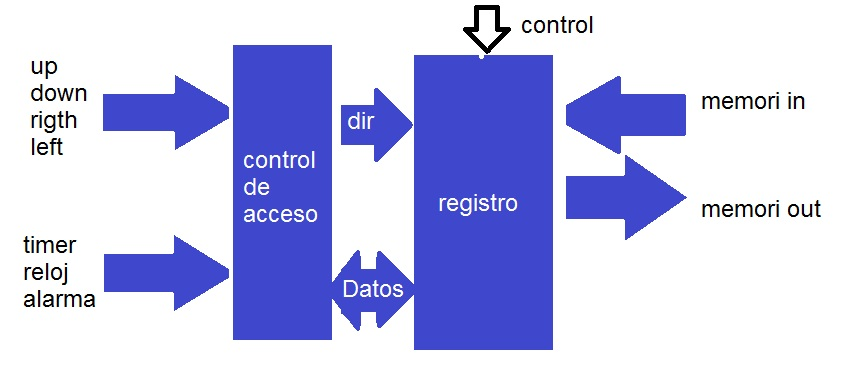
\includegraphics[height=7cm, width=16cm]{img/nivel2_contusr.jpg}
			\caption[1erNivel]{Diagrama de segundo nivel del Teclado.}
			\label{fig:SegundoNivelControlusr}
		\end{figure}
		
		\subsection{Controlador del RTC}
		Para la implementación de esta interfaz que va a permitir la comunicación entre la FPGA y el RTC, se desarrolló 7 bloques principales divididos en una jerarquía de 3 niveles, se puede ver en la figura \ref{fig:Jrtc}. Existen 3 bloques principales uno de inicializacion, un while true, que permite la lectura continua de los datos de la rtc, y una de programación que permite actualizar los cambios del control de usuario, este consta del punto visto anteriormente del control de usurio.\\ [2ex]
		Ademas existen 2 bloques que permiten un bloque que permite leer y escribir datos, esta activa un control que esta basado en los tiempos de la figura \ref{fig:DTE} y la figura \ref{fig:DTL}, como se puede notar existen muchas similitudes entre ambos ciclos, para esto llamaremos a esta diferencia "ciclo" de esta manera podemos armar el cuadro de figura \ref{fig:CTS}\\[2ex]
		Este diagrama muestra los cambios que deben ocurrir según los tiempos del timer dentro del modulo, al llegar el tiempo final saca una bandera indicando el final.\\ [2ex]
		\begin{figure}[htbp]
			\centering
			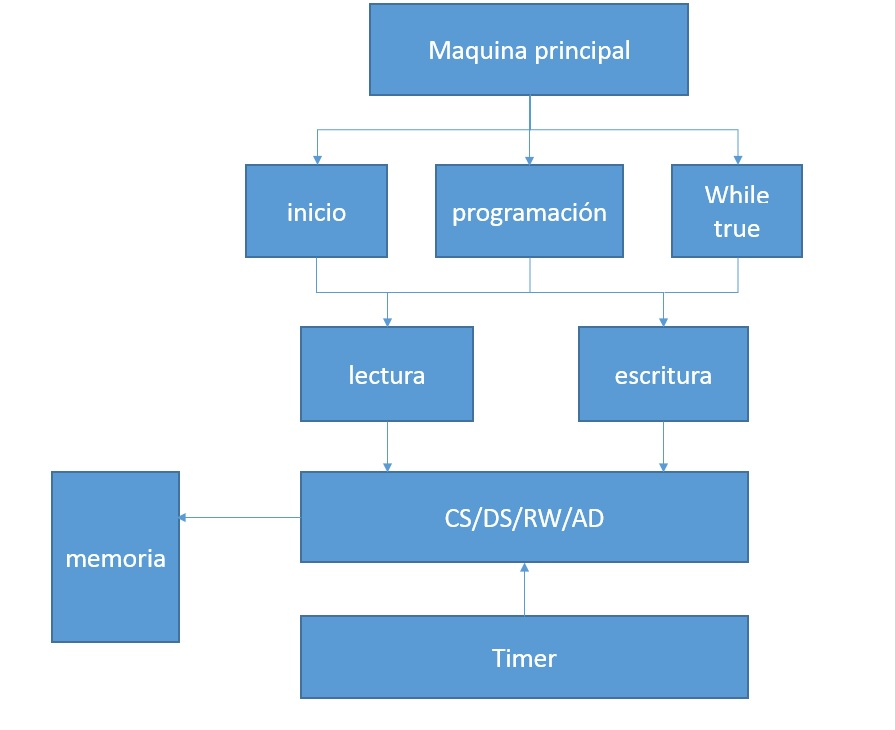
\includegraphics[height=9cm, width=16cm]{img/JerarquiaRTC.jpg}
			\caption[3erNivel]{jerarquía de la RTC.}
			\label{fig:Jrtc}
		\end{figure}
		\begin{figure}[htbp]
			\centering
			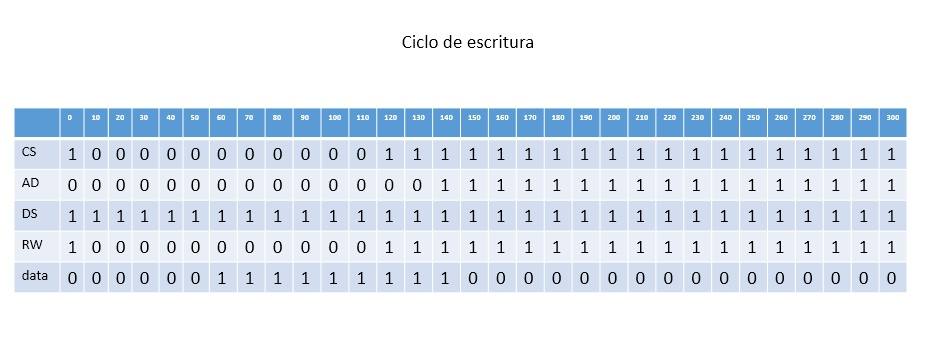
\includegraphics[height=9cm, width=16cm]{img/diagramatiempoescritura.jpg}
			\caption[3erNivel]{Diagrama de tiempos completo del ciclo de escritura.}
			\label{fig:DTE}
		\end{figure}
		\begin{figure}[htbp]
			\centering
			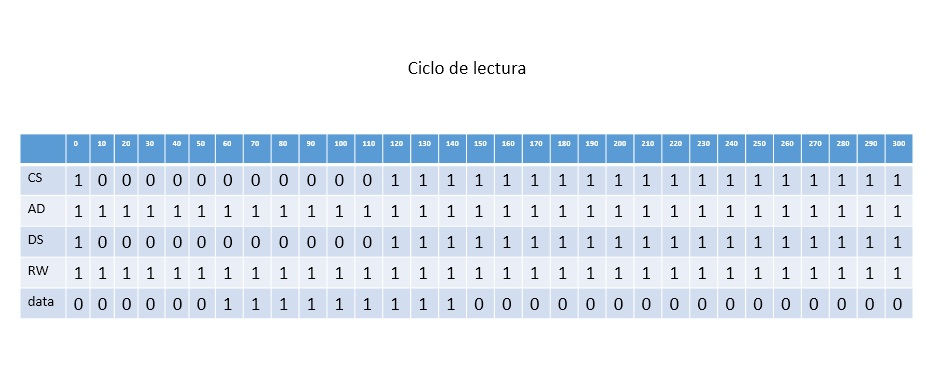
\includegraphics[height=9cm, width=16cm]{img/diagramatiempolectura.jpg}
			\caption[3erNivel]{Diagrama de tiempos completo del ciclo de lectura.}
			\label{fig:DTL}
		\end{figure}
		\begin{figure}[htbp]
			\centering
			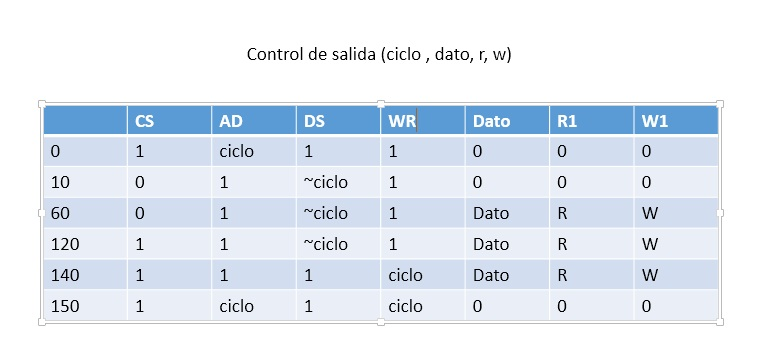
\includegraphics[height=9cm, width=16cm]{img/cuadrotiemposalida.jpg}
			\caption[3erNivel]{cuadro de tiempos del control de salida.}
			\label{fig:CTS}
		\end{figure}
		\subsubsection{nivel 1 control RTC}
		Para este nivel se requiere la entrada y salida de datos al registro de memoria de coneccion y tiene las salidas necesarias para controlar la RTC, esto se nota en la figura \ref{fig:nivel1RTC}.\\[2ex]
		\begin{figure}[htbp]
			\centering
			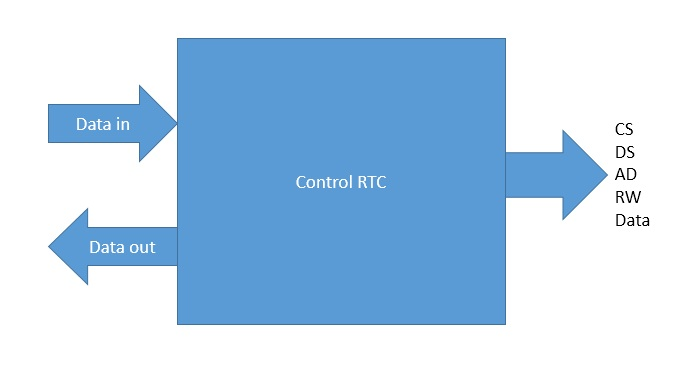
\includegraphics[height=9cm, width=16cm]{img/nivel1_RTC.jpg}
			\caption[3erNivel]{nivel 1 del RTC}
			\label{fig:nivel1RTC}
		\end{figure}
		\subsubsection{nivel 2 RTC}
		Como se menciono antes existen 6 maquina de estados agrupados en 3 jerarquías.\\[2ex]
 		La primera maquina de estados es la de inicializacion, esta tiene un bit de entrada para su inicializacion. Ademas posee salidas de datos y dirección  y bits W y R, que siempre están en cero y se conectan a las maquinas de lectura y escritura respectivamente, esto responde al flujo de la figura \ref{fig:FMEI}.\\[2ex]
		La maquina encargada del proceso while true responde al flujo de la figura, esta tiene un bit para la iniciación de la maquina y un bit que indica que finalizo el proceso, de igual manera un bit que indica que la maquina de estados siguiente termino su proceso para que esta salte entre estados y igual que la maquina pasada tiene las señales W y R y la salida de datos y dirección.\\[2ex]
		Siguiendo la jerarquía, existen 2 maquinas, escritura y lectura, estas respetan los flujos de la figura \ref{fig:FML} y \ref{fig:FME}, estas tienen las entradas de datos y dirección y la señal r y w respectivamente y tiene solo una salida de datos y r y w de esta manera las maquina controla que dato sale, si la direccion y o el dato, ademas tiene el bit de ciclo que determina si esta en el ciclo de escritura o lectura, como se nota en los flujos, el bit de ciclo no depende de la maquina, sino de la parte del programa donde esta se encuentre.\\[2ex]
		Por ultimo el control de salida responde al cuadro de la figura \ref{fig:CTS} a este le entra, el bit de activación que sale de la maquina de escritura o lectura, y entran los datos del ciclo y dato que salen dependiendo del tiempo; internamente este tiene un timer, con el fin de llevar el tiempo desde la activación, y dependiendo del tiempo que transcurre genera los cambios de la figura \ref{fig:CTS}. \\[2ex]
		\begin{figure}[htbp]
			\centering
			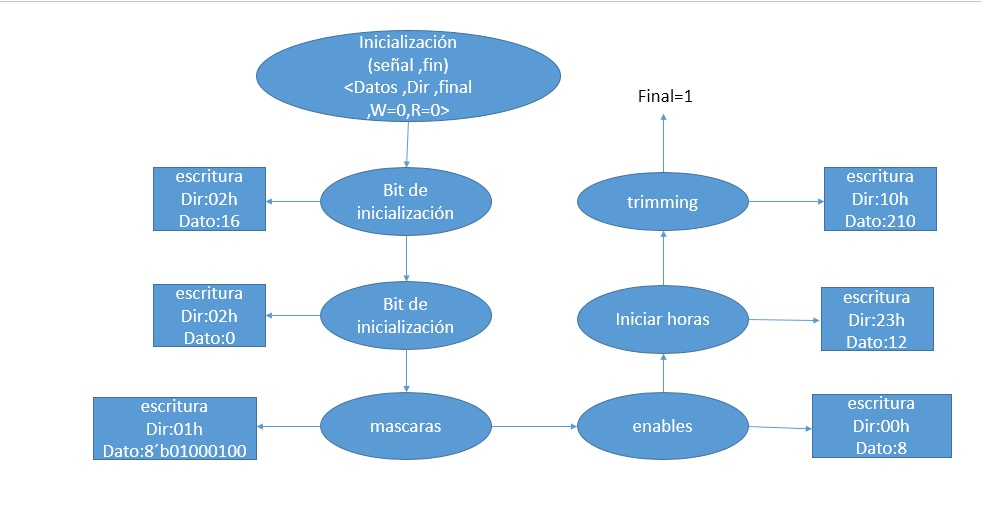
\includegraphics[height=9cm, width=16cm]{img/FlujoInit.jpg}
			\caption[3erNivel]{flujo de datos de la maquina de estados de inicializacion}
			\label{fig:FMEI}
		\end{figure}
		\begin{figure}[htbp]
			\centering
			\includegraphics[height=9cm, width=16cm]{img/FlujoLec.jpg}
			\caption[3erNivel]{flujo de datos de la maquina de lectura}
			\label{fig:FML}
		\end{figure}
		\begin{figure}[htbp]
			\centering
			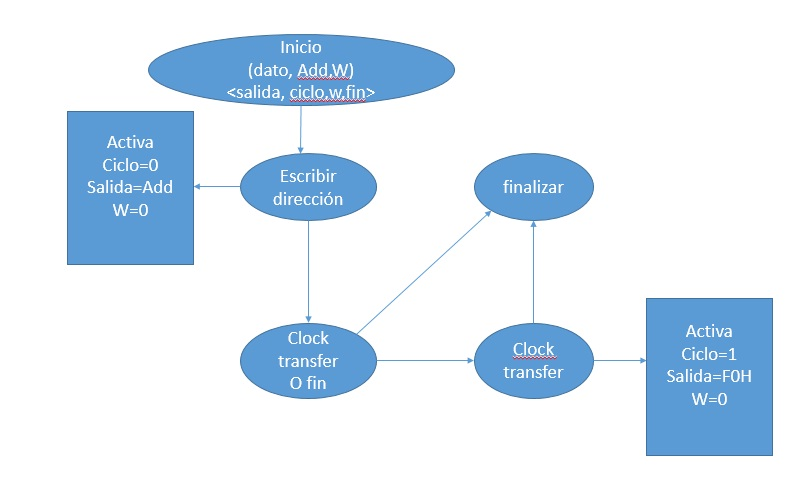
\includegraphics[height=9cm, width=16cm]{img/FlujoEsc.jpg}
			\caption[3erNivel]{flujo de datos de la maquina de Escritura}
			\label{fig:FME}
		\end{figure}
		\subsection{Control general de la RTC}
		
		Debido a que existen muchas maquinas con diferentes jerarquia se ocupa diseñar una maquina de estado genral que controle y vigile el funcionamiento entre la maquinas de estados.
		Esta maquina posee 5 niveles la inicializacion de la RTC, la inicializacion de la RTC en cero, el inico de lectura continua, la solicutud de escritura y la escritura de los cambios en la memoria.
		
		\subsubsection{inicializacion}
		
		Este consta del primer estado del control de la RTC, este estado consta de los parametros de e instrucciones que deban introducirse en la RTC para que esta comience a correr el tiempo, ademas de la escriura de la mascaras en los estados 0 y 1 de la RTC, que nos permiten poner las banderas del timer y iniciar con el cronometro detenido.
		Aparte de ser el estado inicial de toda la RTC, este es el estodo donde este vuelve cada vez que es reinicia.
		
		\subsubsection{inicializacion de la memoria en cero}
		
		El objetivo de este estado es que todos los datos de la memoria inicie en valores conocidos cada vez que se reinicia o inicia la RTC. Para este efecto se aprovechara el efecto de escritura en la rtc que tiene el control de usuario. 
		Como el control de usuario escribe lo que este en la memoria, mas un cambio en la RTC, en la RTC. Si no existe cambios en la memoria en la RTC se escribiran los valore iniciales de la memoria, como esta inicia en cero, la RTC iniciara a contar desde cero.
		
		\subsubsection{lectura continua}
		
		 Este bloque es el que lee los valores que se encuentra cambiando en la RTC, este es el modulo que actualiza constantemente los valores de la RTC en la memoria dentro de la FPGA.
		 Este estado genera una pausa mientras la memoria se estabiliza para mea estados. 
		
		\subsubsection{solicitud de control de usuario}
		
		Para controlar la escritura en el control de usuario no se escribirá dentro de la RTC todo el tiempo, solo cuando termine el ciclo de lectura continua y el usurario este realizando cambios, este es un estado transitorio, en este estado puede pasar al estado de lectura continua o a la escritura de cambios
		
		\subsubsection{escritura de cambios}
		
		Esta etapa activa el control de usuario para poder alterar los valores de la RTC con los valores que el usuario desea alterar. Esta estap solo se accede cuando el usurio desea realizar cambios en la RTC.
		
		
		\section{Datos y resultados}
		\subsection{Simulaciones}
		
		
		\section{Análisis de datos y resultados}
		
		
		\section{Hoja de datos de unidades desarrolladas}
		
		
		\section{Conclusiones y recomendaciones}
		\subsection{Conclusiones}
		
		
		\subsection{Recomendaciones}
		
		
	\end{document}
